
El componente utilizado para ampliar la señal enviada por el Arduino al motor, sirviendo de intermediario entre éste y los motores, es el módulo de control PWM de motores con un circuito integrado LMD18200T que soporta hasta tres Amperios. Es un puente H controlado por PWM. Satisface los requisitos necesarios en nuestra tarea: Precio, voltaje, amperaje y de implementación sencilla. Se aprecian en la~\cref{fig:Hbridge} las entradas y las salidas de las que dispone. De arriba abajo y de izquierda a derecha disponemos de:

\begin{itemize}
	\item \textbf{GND:} La tierra de la placa de control, en nuestro caso el Arduino.
	\item \textbf{PWM(Pulse width modulation):} la señal del control por ancho de pulsos.
	\item \textbf{Dir:} Señal con el sentido de giro que se desea.
	\item \textbf{Brake:} Freno del motor
	\item \textbf{V+:} Alimentación de 12 voltios.
	\item \textbf{GND:} tierra.
	\item \textbf{OUT1:} Salida de una mitad del puente H.
	\item \textbf{OUT2:} Salida de la otra mitad del puente H
\end{itemize}

El esquema final de conexión entre raspberry, puente H y motor lo podemos contemplar en la~\cref{fig:conectionDiagram}\\

\begin{figure}[H]
		\centering
		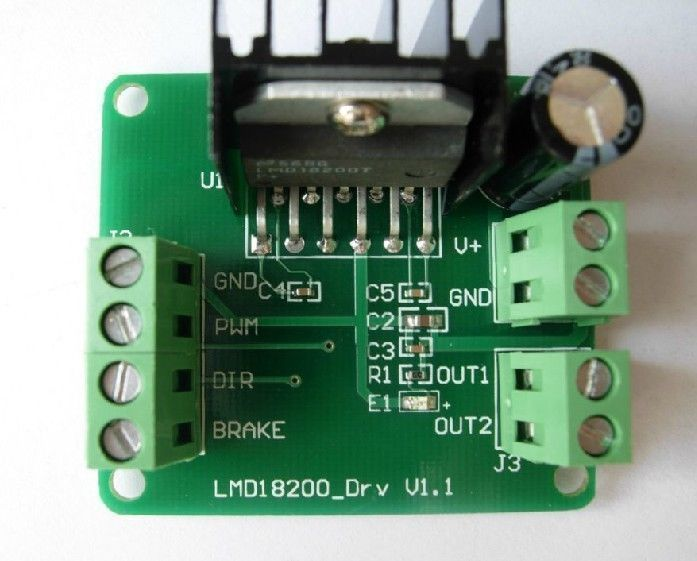
\includegraphics[scale = 0.3]{part/Proyecto_ejecutivo/memoria_constructiva/motor/img/modulopot}
		\caption{Módulo de potencia}\label{fig:Hbridge}
\end{figure}

\begin{figure}[H]
		\centering
		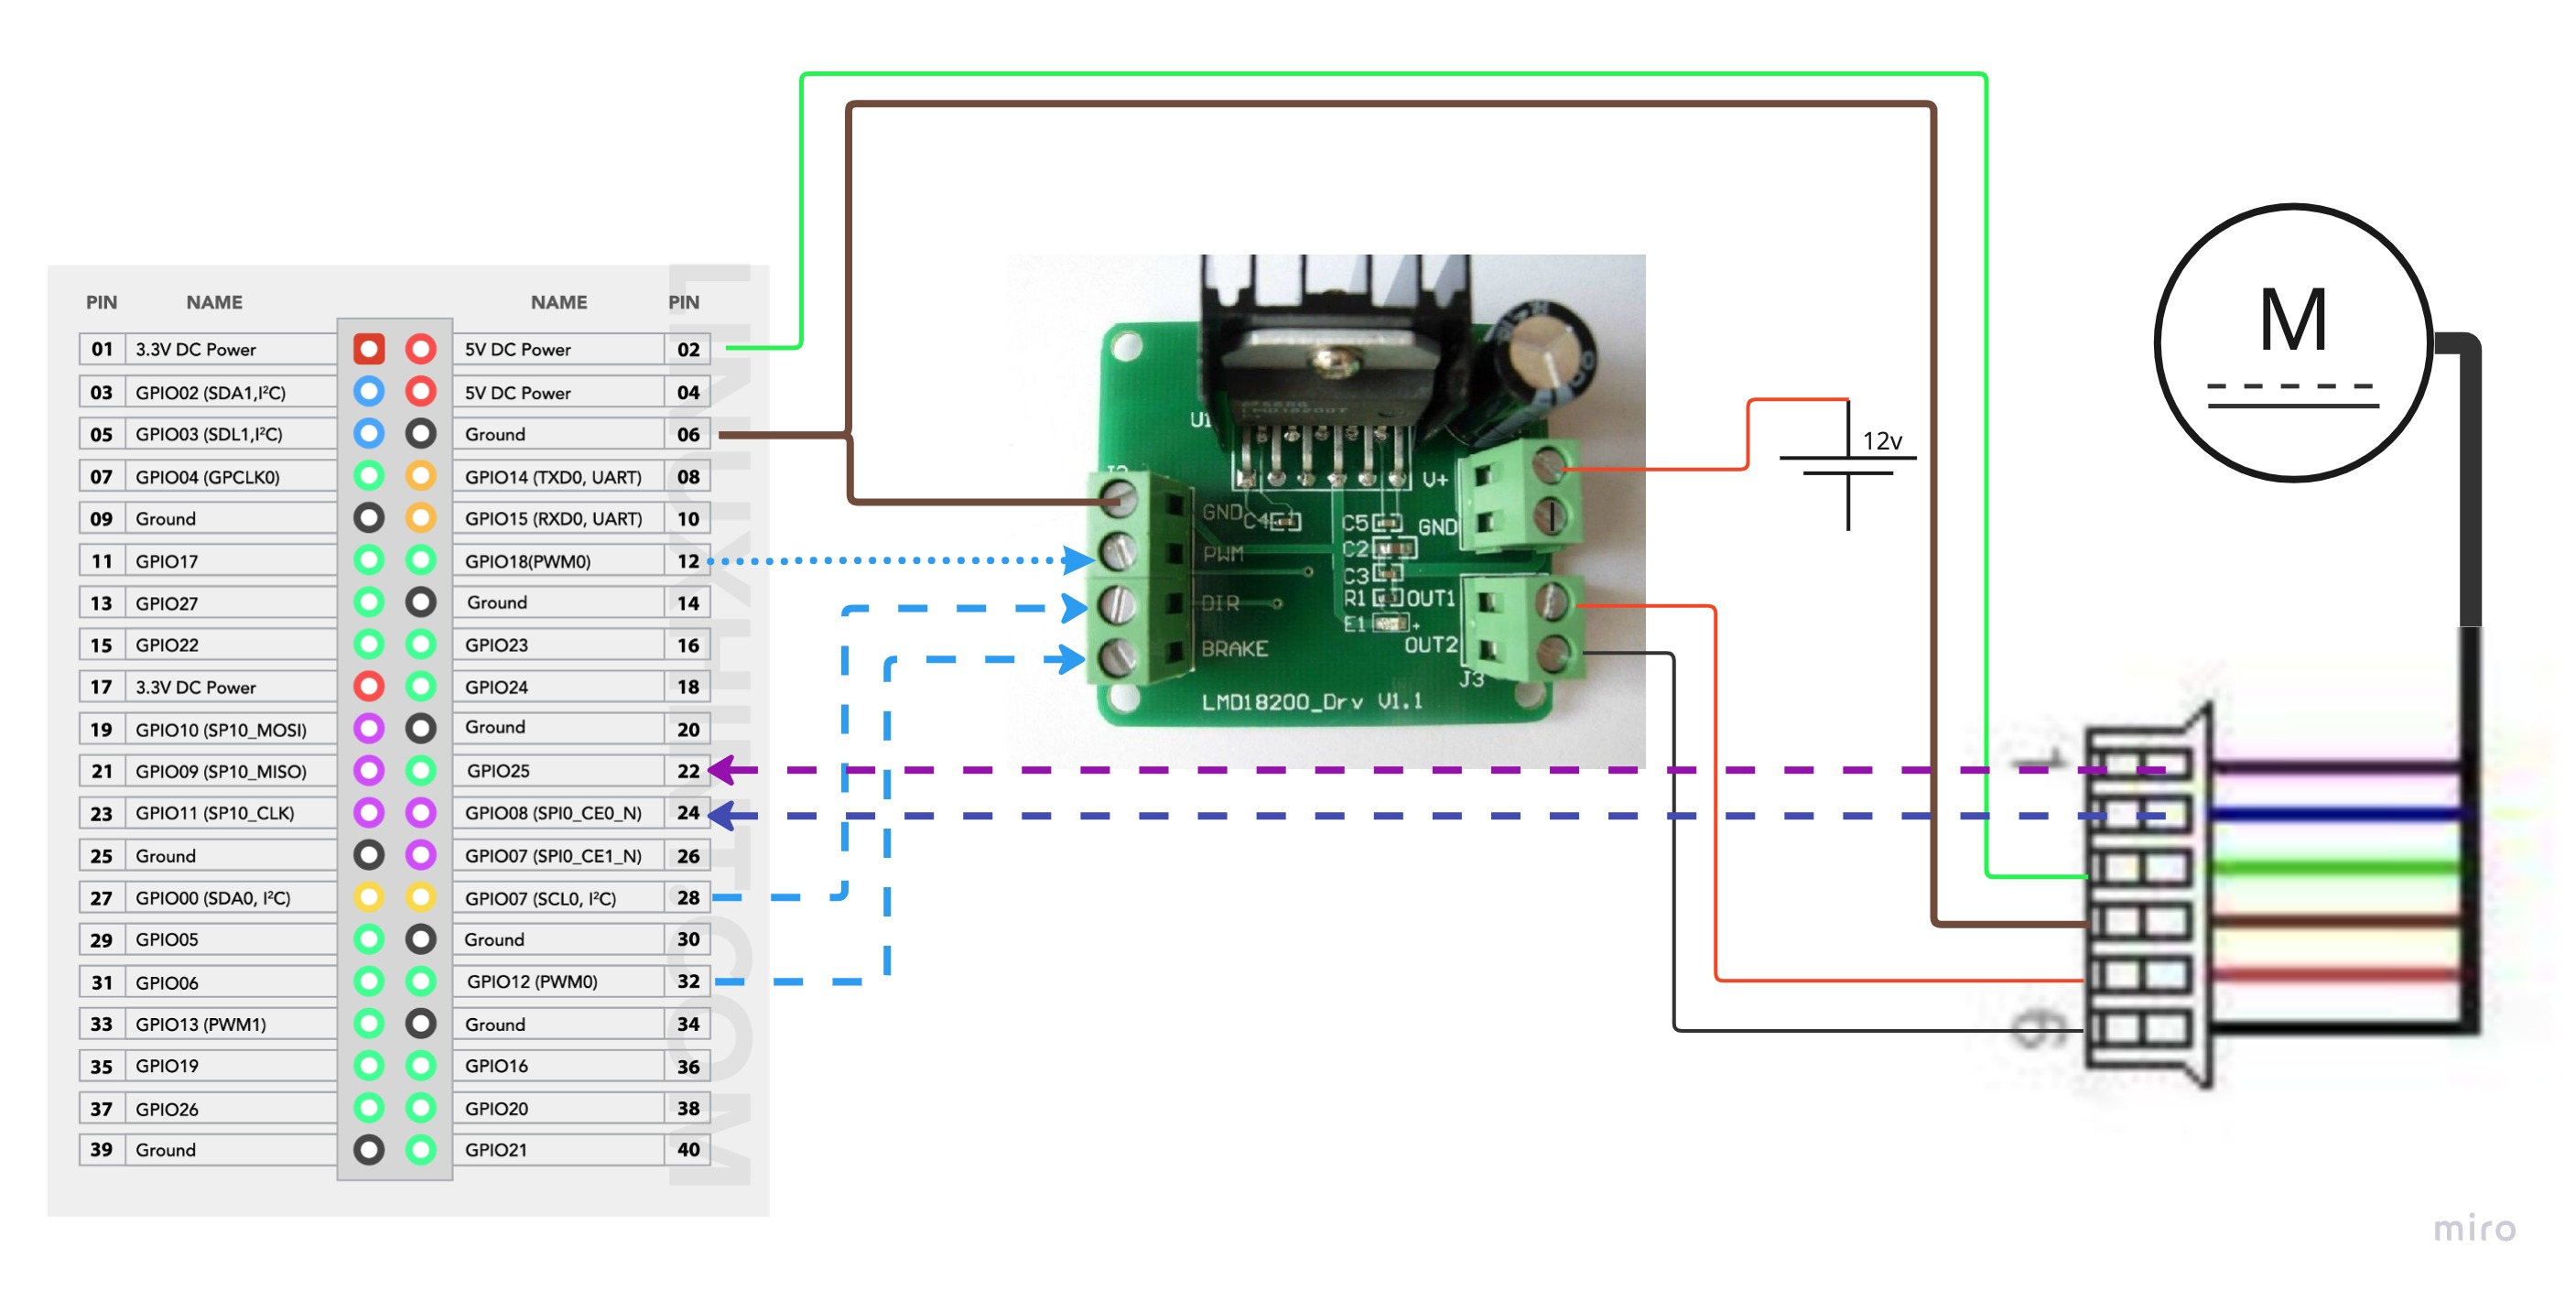
\includegraphics[scale = 0.15]{part/Proyecto_ejecutivo/memoria_constructiva/motor/img/connection diagram}
		\caption{Esquema de conexión del módulo de potencia.\\Fuente: elaboración propia.}\label{fig:conectionDiagram}
\end{figure}